\documentclass[12pt]{article}

% packages :
\usepackage[utf8x]{inputenc}
\usepackage[T1]{fontenc}
%\usepackage[francais]{babel}
%
\usepackage{graphicx} % images
\usepackage{float}
\usepackage{placeins}
\usepackage{multirow}
\usepackage{wrapfig}
\usepackage{array}

\usepackage{xparse}
\usepackage{tikz}

\usepackage[top=2cm, bottom=2cm, left=2.5cm, right=2.5cm]{geometry}


% maths :
\usepackage{amsthm}
\usepackage{amsmath}
\usepackage{amssymb}
\usepackage{mathrsfs}

\begin{document}

% CODE POUR LES MAPS DE KARNAUGH
% (réécriture en Tikz de https://www.ctan.org/tex-archive/macros/latex/contrib/karnaugh)

\newlength{\kmapbasesize}
\setlength{\kmapbasesize}{1cm}
\def\kmaptspanning{0.04}

\newcommand{\kmapbox}[4]{\draw[kstyle,rounded corners=\rcorner] (#1 * \kmapbasesize + \kmaptspanning * \kmapbasesize,#2  * \kmapbasesize - \kmaptspanning * \kmapbasesize) rectangle +(#3 * \kmapbasesize - 2 * \kmaptspanning * \kmapbasesize,#4  * \kmapbasesize + 2*\kmaptspanning * \kmapbasesize)}

\NewDocumentCommand{\kmtake}{omm}{
\IfNoValueF{#1}{\tikzset{kstyle/.style={#1}}}
\pgfmathsetmacro{\rcorner}{min(#3) > 1 ? \kmapbasesize : .5 * \kmapbasesize}
\pgfmathsetmacro{\x}{array({#2},0)}
\pgfmathsetmacro{\y}{-array({#2},1)}
\pgfmathsetmacro{\w}{array({#3},0)}
\pgfmathsetmacro{\h}{-array({#3},1)}
\begin{scope}
\clip (0,0) rectangle +(\nLineX * \kmapbasesize, -\nLineY * \kmapbasesize);
\kmapbox{\x}{\y}{\w}{\h};
% extra!
\pgfmathparse{array({#2},0) + array({#3},0) > \nLineX}
\if\pgfmathresult1
\pgfmathsetmacro{\nx}{\x - \nLineX}
\kmapbox{\nx}{\y}{\w}{\h};
\fi
\pgfmathparse{array({#2},1) + array({#3},1) > \nLineY}
\if\pgfmathresult1
\pgfmathsetmacro{\ny}{\y + \nLineY}
\kmapbox{\x}{\ny}{\w}{\h};
\fi
\pgfmathparse{and(array({#2},0) + array({#3},0) > \nLineX, array({#2},1) + array({#3},1) > \nLineY)}
\if\pgfmathresult1
\pgfmathsetmacro{\nx}{\x - \nLineX}
\pgfmathsetmacro{\ny}{\y + \nLineY}
\kmapbox{\nx}{\ny}{\w}{\h};
\fi
\end{scope}
}

\NewDocumentCommand{\kmap}{mmo}{
\def\args{{#1}}

\pgfmathsetmacro{\numVar}{dim(\args)}
\pgfmathsetmacro{\numVarm}{\numVar - 1}
\pgfmathsetmacro{\nVarX}{int(ceil(\numVar / 2))}
\pgfmathsetmacro{\nVarXm}{\nVarX - 1}
\pgfmathsetmacro{\nVarY}{int(\numVar - \nVarX)}
\pgfmathsetmacro{\nVarYm}{\nVarY - 1}
\pgfmathsetmacro{\nLineX}{2 ^ \nVarX}
\pgfmathsetmacro{\nLineXm}{\nLineX - 1}
\pgfmathsetmacro{\nLineY}{2 ^ \nVarY}
\pgfmathsetmacro{\nLineYm}{\nLineY - 1}

% draw table
\foreach\i in {0,...,\nLineX}{
	\draw (\i * \kmapbasesize,0) -- +(0,- \nLineY * \kmapbasesize);
}

\foreach\i in {0,...,\nLineY}{
	\draw (0,- \i * \kmapbasesize) -- +(\nLineX * \kmapbasesize,0);
}

% add variables
\pgfmathsetmacro{\smm}{.003 * \kmapbasesize}
\foreach\i in {0,...,\nVarXm}{
	\draw (\i * \kmapbasesize, .25 * \kmapbasesize + .6 * \i * \kmapbasesize)  ++(0,-\smm) -- ++(0, 2 * \smm)  ++(0,-\smm) -- node[above,midway]{\pgfmathparse{\args[\i]}\pgfmathresult} ++(\kmapbasesize * 2 ^ \nVarXm, 0) ++(0,-\smm) -- ++(0, 2 * \smm)  ++(0,-\smm);
}

\pgfmathparse{\nVarY > 0}\if\pgfmathresult1
\foreach\i in {0,...,\nVarYm}{
	\draw ( - .25 * \kmapbasesize - .7 * \i * \kmapbasesize, - \i * \kmapbasesize ) ++(-\smm,0) -- ++(2 * \smm,0)  ++(-\smm,0) -- node[left,midway]{\pgfmathparse{\args[\nVarX + \i]}\pgfmathresult} ++(0, - \kmapbasesize * 2 ^ \nVarYm)   ++(-\smm,0) -- ++(2 * \smm,0)  ++(-\smm,0);
}\fi

%% write
\foreach\i in {0,...,\nLineXm}{
	\foreach\j in {0,...,\nLineYm}{
		\pgfmathsetmacro{\val}{int(\j * \nLineX + \i)}
		\draw (\i * \kmapbasesize, - \j * \kmapbasesize) node[anchor=north west] {\tiny \foreach\k in {0,...,\numVarm} {\pgfmathsetmacro{\ok}{\k - \nVarX}\pgfmathparse{\k < \nVarX ? (and(\i - \k < \nLineX / 2, notless(\i, \k)) ? 1 : 0) : (and(\j - \ok < \nLineY / 2, notless(\j, \ok)) ? 1 : 0)}\pgfmathresult}};
		\draw (\i * \kmapbasesize + .5 * \kmapbasesize, - \j * \kmapbasesize - .6 * \kmapbasesize) node{\pgfmathparse{array({#2},\val)}\pgfmathresult};
	}
}
}

% CODE POUR L'AFFICHEUR 7 SEGMENTS
% (inspiré de http://sciences-indus-cpge.papanicola.info/Afficheur-7-Segments-avec-PGF-TIKZ)

\tikzstyle SSGOn=[fill=red]
\tikzstyle SSGOff=[fill=gray!50!black]

\newlength{\SSGBarThickness}
\setlength{\SSGBarThickness}{4pt}
\newlength{\SSGTri}
\setlength{\SSGTri}{2pt}
\newlength{\SSGPad}
\setlength{\SSGPad}{1pt}

\newcommand{\SSdbar}[4]{
\pgfmathsetmacro{\bstyle}{#1 == 1 ? "SSGOn" : "SSGOff"}
\pgfmathsetmacro{\rto}{#4 == 0 ? 0 : 90}
\pgfmathsetmacro{\px}{array({#2},0)}
\pgfmathsetmacro{\py}{array({#2},1)}
\begin{scope}[xshift=\px,yshift=\py]
\begin{scope}[rotate=\rto]
\path[\bstyle] (\SSGTri+\SSGPad,-\SSGBarThickness / 2) -- (\SSGPad, 0) -- (\SSGTri+\SSGPad,\SSGBarThickness / 2) -- ++(#3 - 2*\SSGPad - 2*\SSGTri, 0) -- ++ (\SSGTri,-\SSGBarThickness / 2) -- (#3 -\SSGPad-\SSGTri,-\SSGBarThickness / 2) -- cycle;
\end{scope}
\end{scope}	
}

\NewDocumentCommand{\SSdx}{omm}{
\pgfmathsetmacro{\cpx}{array({#2},0)}
\pgfmathsetmacro{\cpy}{array({#2},1)}
\def\csz{\IfNoValueTF{#1}{1em}{#1}}
\begin{scope}[xshift=\cpx cm - \csz / 2,yshift=\cpy cm]
\pgfmathparse{array({#3},0)}
\SSdbar{\pgfmathresult}{0,\csz}{\csz}{0} % a
\pgfmathparse{array({#3},1)}
\SSdbar{\pgfmathresult}{\csz,0}{\csz}{1} % b
\pgfmathparse{array({#3},2)}
\SSdbar{\pgfmathresult}{\csz,-\csz}{\csz}{1} % c
\pgfmathparse{array({#3},3)}
\SSdbar{\pgfmathresult}{0,-\csz}{\csz}{0} % d
\pgfmathparse{array({#3},4)}
\SSdbar{\pgfmathresult}{0,-\csz}{\csz}{1} % e
\pgfmathparse{array({#3},5)}
\SSdbar{\pgfmathresult}{0,0}{\csz}{1} % f
\pgfmathparse{array({#3},6)}
\SSdbar{\pgfmathresult}{0,0}{\csz}{0} % g
\end{scope}
}

\NewDocumentCommand{\SSdn}{omm}{
\if#30
\SSdx[#1]{#2}{1111110}
\fi
\if#31
\SSdx[#1]{#2}{0110000}
\fi
\if#32
\SSdx[#1]{#2}{1101101}
\fi
\if#33
\SSdx[#1]{#2}{1111001}
\fi
\if#34
\SSdx[#1]{#2}{0110011}
\fi
\if#35
\SSdx[#1]{#2}{1011011}
\fi
\if#36
\SSdx[#1]{#2}{1011111}
\fi
\if#37
\SSdx[#1]{#2}{1110000}
\fi
\if#38
\SSdx[#1]{#2}{1111111}
\fi
\if#39
\SSdx[#1]{#2}{1111011}
\fi
}

% LES TABLEAUX ET 7 SEGMENTS

\begin{center}
\begin{tikzpicture}
\kmap{"$a$", "$b$", "$c$"}{%
"","","","",%
"","","","",}
\end{tikzpicture}

\begin{tikzpicture}
\kmap{"$a$", "$b$", "$c$", "$d$"}{%
"","","","",%
"","","","",%
"","","","",%
"","","","",%
}
\end{tikzpicture}
\end{center}

\begin{center}
\begin{tikzpicture}
\kmap{"$a$", "$b$", "$c$"}{%
1,0,0,0,%
1,1,0,0}
\end{tikzpicture}

\begin{tikzpicture}
\kmap{"$a$", "$b$", "$c$"}{%
1,0,0,0,%
1,1,0,0}{
\kmtake[green!50!black]{0,0}{1,2}
\kmtake[blue]{0,1}{2,1}
}
\end{tikzpicture}

\begin{tikzpicture}
\kmap{"$a$", "$b$", "$c$"}{%
1,0,0,0,%
1,1,0,0}{
\kmtake[orange]{1,0}{2,1}
\kmtake[magenta]{2,0}{2,2}
}
\end{tikzpicture}
\end{center}


\begin{center}
\begin{tikzpicture}
\kmap{"$a$", "$b$", "$c$", "$d$"}{%
1,0,1,1,%
0,0,0,1,%
1,0,0,1,%
1,0,1,1,%
}
\end{tikzpicture}

\begin{tikzpicture}
\kmap{"$a$", "$b$", "$c$", "$d$"}{%
1,0,1,1,%
0,0,0,1,%
1,0,0,1,%
1,0,1,1,%
}{
\kmtake[green!50!black]{2,3}{2,2}
\kmtake[blue]{3,2}{2,2}
}
\end{tikzpicture}

\begin{tikzpicture}
\kmap{"$a$", "$b$", "$c$", "$d$"}{%
1,0,1,1,%
0,0,0,1,%
1,0,0,1,%
1,0,1,1,%
}{
\kmtake[green!50!black]{2,3}{2,2}
\kmtake[blue]{3,2}{2,2}
\kmtake[magenta,thick]{3,0}{1,4}
\kmtake[orange,thick]{3,3}{2,2}
}
\end{tikzpicture}
\end{center}

\begin{center}
\begin{tikzpicture}
\kmap{"$a$", "$b$", "$c$", "$d$"}{%
1,0,1,1,%
0,0,0,1,%
1,0,0,1,%
1,0,1,1,%
}{
\kmtake[green!50!black]{1,1}{2,2}
\kmtake[blue]{1,0}{1,4}
\kmtake[magenta]{0,1}{2,1}
}
\end{tikzpicture}


\vspace*{2cm}
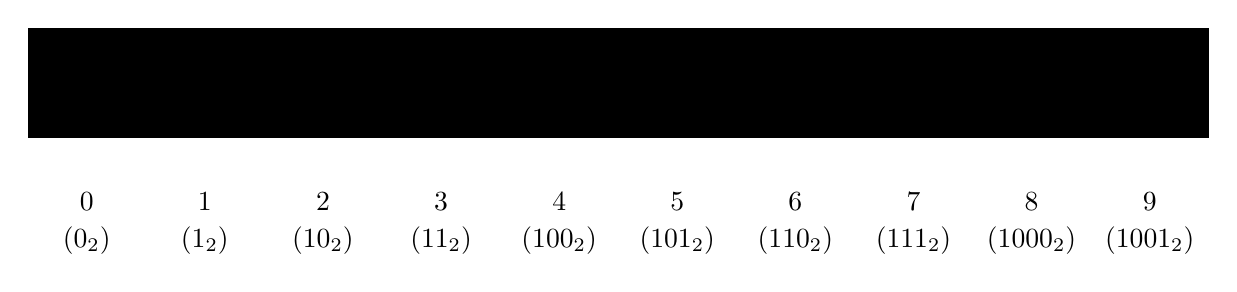
\begin{tikzpicture}
\fill[black] (-.75,-2em) rectangle +(15,4em);
\foreach\i in {0,...,9} {
\SSdn[1.5em]{\i*1.5,0}{\i}
\draw (\i*1.5,-1.5) node {\i};
\draw (\i*1.5, -2) node { (\pgfmathbin{\i}$\pgfmathresult_2$)};
}
\end{tikzpicture}

\vspace{2cm}
\begin{tikzpicture}
\tikzstyle SSGOff=[draw]
\setlength{\SSGBarThickness}{16pt}
\setlength{\SSGTri}{8pt}
\setlength{\SSGPad}{4pt}
\SSdx[5em]{0,0}{0000000}
\draw (0,0) node {G};
\draw (0,5em) node {A};
\draw (0,-5em) node {D};
\draw (-2.5em,2.5em) node {F};
\draw (2.5em,2.5em) node {B};
\draw (-2.5em,-2.5em) node {E};
\draw (2.5em,-2.5em) node {C};
\end{tikzpicture}
\end{center}

\begin{center}
\begin{tikzpicture}
\kmap{"$a_1$", "$a_2$", "$a_3$", "$a_4$"}{%
"X","X",1,1,%
"X","X",0,1,%
1,"X",1,0,%
1,"X",1,0,%
}{
%\kmtake[green!50!black]{2,3}{2,2}
}
\end{tikzpicture}

\begin{tikzpicture}
\kmap{"$a_1$", "$a_2$", "$a_3$", "$a_4$"}{%
"X","X",1,1,%
"X","X",0,1,%
1,"X",1,0,%
1,"X",1,0,%
}{
\kmtake[green!50!black]{0,0}{2,4}
\kmtake[blue]{3,0}{2,2}
\kmtake[magenta]{0,0}{4,1}
\kmtake[orange]{1,2}{2,2}
}
\end{tikzpicture}
\end{center}

\begin{center}


\begin{tikzpicture}
\kmap{"$a_1$", "$a_2$", "$a_3$", "$a_4$"}{%
"X","X",1,1,%
"X","X",0,1,%
1,"X",1,0,%
1,"X",1,0,%
}{
\kmtake[green!50!black]{0,0}{2,4}
\kmtake[blue]{3,0}{2,2}
\kmtake[magenta]{0,0}{4,1}
\kmtake[orange]{1,2}{2,2}
}
\end{tikzpicture}\hspace*{1cm}
\begin{tikzpicture}
\kmap{"$a_1$", "$a_2$", "$a_3$", "$a_4$"}{%
"X","X",1,1,%
"X","X",0,1,%
1,"X",1,0,%
1,"X",1,0,%
}{
\kmtake[green!50!black]{0,0}{2,4}
\kmtake[blue]{3,0}{2,2}
\kmtake[magenta]{1,3}{2,2}
\kmtake[orange]{1,2}{2,2}
}
\end{tikzpicture}
\end{center}


\end{document}